\section{Introduction}
\label{sec:introduction}
% state the learning objective

\par The objective of this laboratory assignment is to study a circuit containing a capacitor and a sinusoidal voltage source $v_s$.The value of this sinusoidal voltage source varies in time according to the following equations: 
\begin {equation}
	v_s( t)  = V_s u(-t) + sin( 2 \pi f t ) u( t)
	\label{eq:i1}
\end{equation}
 with 
\begin {equation}
	u( t ) =  
	\begin{cases*} 
	  0 & if $t < 0$ \\
	1, & if $t \geq 0$
	\end{cases*}
	\label{eq:i2}
\end{equation}

In this circuit there is also a linearly dependent voltage and current source. The circuit also contains 7 resistors.\par
The nodes of the circuit were numbered arbitrarily (from {\it$V_{0}$}  to {\it$V_{7}$} ), and it was considered that {\it node 0} was the ground node. The voltage-controlled current source {\it $I_b$} has a linear dependence on Voltage {\it $V_b$}, of constant {\it $K_b$}. The voltage {\it $V_b$} is the voltage drop at the ends of resistor {\it $R_3$}. The current-controlled voltage source {\it $V_d$} has a linear dependece on current {\it $I_d$}, of constant {\it $K_d$}. The control current {\it $I_d$} is the current that passes through the resistor {\it $R_6$}.
The circuit can be seen in \textbf{Figure~\ref{fig:circuit_t2}}.\par
%The values for the resistors and the  constants for the dependent 
%sources are presented in \textbf{Table~\ref{tab:python_values}}. 
These values for the capacitance, resistors and the constants for the dependent sources were obtained using the
Python script provided by the Professor 
and using the number 95815 as the seed.The seed number can be altered in the top Makefile (line 9). By doing so, all figures and tables will be updated acording to the new values. \par

In Section~\ref{sec:analysis}, a theoretical analysis of the circuit is
presented. Here the circuit is analised for $t<0$ using the nodal analysis and the equivalent resistence $R_{eq}$ as seen from the capacitor terminals is determined. In this section both the natural and forced solutions for $V_6$ are also determined as well as the frequency responses for $V_c, V_s$ and $V_6 $. In Section~\ref{sec:simulation}, the circuit is analysed by
simulation using the program Ngspice. An operating point analysis is used to analyse the circuit when $t<0$ and another one to determine the time constant.A transient analysis is used to determine the natural and forced responses on node 6. A frequency analysis is also performed on node 6. The conclusions of this study are outlined in
Section~\ref{sec:conclusion}, where the theoretical results obtained in
Section~\ref{sec:analysis} are compared to the simulation results obtained in
Section~\ref{sec:simulation}.

\begin{figure}[h] \centering
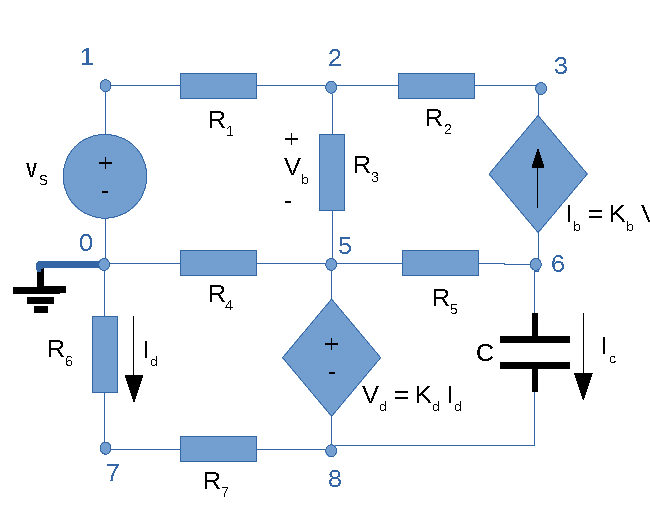
\includegraphics[width=0.6\linewidth]{circuit_t2.pdf}
\caption{Circuit in study}
\label{fig:circuit_t2}
\end{figure}


%\begin{table}[h]
% \centering
 % \begin{tabular}{|l|r|}
  %  \hline    
   % {\bf Name} & {\bf Python-generated values} \\ \hline
	%R1 &  1.04606282456 \\ \hline
	%R2 &  2.00732621328 \\ \hline
	%R3 &  3.06060705885 \\ \hline
	%R4 &  4.07055531265 \\ \hline
	%R5 &  3.1225213804 \\ \hline
	%R6 &  2.06927045958 \\ \hline
	%R7 &  1.01531018068 \\ \hline
	%Va &  5.24359648479 \\ \hline
	%Id &  1.01891541651 \\ \hline
	%Kb &  7.0473187437 \\ \hline
	%Kc &  8.3479788681 \\ 
	%\hline

  %\end{tabular}
  %\caption{The variables that start with an {\it R} are the values of the resistors 
    %and are expressed in  kiloohm  (kOhm); the variable {\it Va} is a {\it voltage} and is expressed in
    %Volt (V) and the variable {\it Id}  is a {\it current} and expressed in
   %miliAmpere (mA). The constants {\it Kc} and {\it Kb} are  expressed in
   %kiloOhm  (kOhm) and miliSiemens (mS), respectively.}
  %\label{tab:python_values}
%\end{table}


\pagebreak

